\subsection{RQ2: Does advice change actions and outcomes?}
\label{sec:behavior}
At the intervention query, all 869 eligible pairs have identical recorded state and RGB hashes, different instruction hashes, and immediately different returned action hashes. The action hash covers the returned array's shape, dtype, and bytes; it does not include the instruction. Thus zero-step action-output divergence is observed in all 56 rescued and all 813 non-rescued pairs, with no missing trigger record. This establishes a computational difference, not its magnitude or usefulness. Hashes cannot distinguish a meaningful motor correction from a tiny numerical perturbation, and this comparison does not independently randomize service scheduling or arithmetic effects.

To measure recovery timing, define $u_i=(T_i-\tau_i)/(H_i-\tau_i)$ for a rescued pair, where $T_i$ is its recorded success step. Figure~\ref{fig:timing} plots
\begin{equation}
G_E(u)=\frac{1}{869}\sum_{i:R_i=1}\ind[u_i\leq u],
\end{equation}
with zero contribution from non-rescues. Unlike a CDF conditioned only on success, this curve retains all eligible failures in its denominator and ends at 6.44\%, not 100\%.

\begin{figure}[t]
\centering
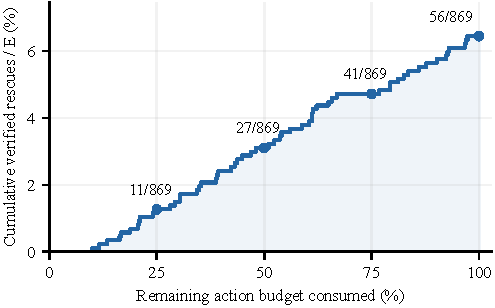
\includegraphics[width=\columnwidth]{figures/recovery_timing.pdf}
\caption{\textbf{Recovery takes continued action.} At 25/50/75/100\% of the remaining budget, 11/27/41/56 cases have succeeded, out of 869 eligible pairs. All 813 eligible non-rescues reach their original horizons. The curve describes recorded success timing, not performance under alternative intervention times.}
\label{fig:timing}
\end{figure}

Among the 56 rescues, median $u_i$ is 51.67\% (interquartile range 30.45--77.41\%), and the median continuation is 361 environment steps. Fifteen rescues finish in the last quarter of their remaining budget; seven use more than 90\%. A short observation window after advice would therefore miss recorded successes. An earlier trigger might help, harm, or leave outcomes unchanged; that counterfactual has not been tested.
